% Drawing 154/08-21 -- folder 154, batch 08, archive page 147 (PDF page 148).
% Transcription: grand dessin à l'encre et au crayon : un disque aux deux pôles marqués (en haut et en bas), joints par un faisceau de fines courbes (un balayage), traversé de pseudo-droites ; un réseau de flèches (noires et brunes) va de croisement en croisement, les sommets numérotés de $1$ à $19$ ; plusieurs numéros sont groupés et entourés ; en haut à droite, « $17 = 1$ ». Des régions hachurées au bord. En bas à droite, un petit disque au crayon rempli d'un réseau de flèches ; en haut à droite, un croisement de trois droites sur une droite hachurée
% Kind: disk with a sweep and a network of numbered arrows. Method 2 (schematic redraw from the facsimile). Status: partial.
% Notes: Whole-page figure of great density, redrawn as a skeleton only. Drawn: the pencil rim, the two poles and six curves of the sweep, the vertex 1 at the left with its two arrows, a selection of the thick arrows of the network (the chain along the upper left, the star in the upper middle, the long arrows to the right and to the lower right), the circled groups « 1, 2, 3, 4 », « 18, 19 » (twice) and the mention 17 = 1; at the right, the three lines crossing on a marked point of a fourth line, and the small pencil disk (drawn empty). Not drawn: the pseudo-lines themselves, most of the arrows, the numbers of the vertices, the hatched regions, the network inside the small disk. The arrows drawn are placed from a page view and show the layout, not the incidences. Redrawn 2026-11-12 (issue 128): to check again.
% Coordinates: 1 unit = 1 mm = 1/100 of the crop width (bbox in page fractions: [0.21, 0.085, 0.9, 0.465]).
% Redrawn by Claude (claude-fable-5-2), issue #128, 2026-11-12; not checked by a human; not compiled (no TeX in the session).
% Rights: reproduces part of the work -- behind RENDER_TRANSCRIPTS, never published by itself.
\documentclass[tikz,border=3pt]{standalone}
\usepackage{amsmath,amssymb}
\usetikzlibrary{patterns,arrows.meta}
\tikzset{pencil/.style={black!45}, struck/.style={black!35}, mpt/.style={circle,draw,inner sep=1.3pt}, pt/.style={circle,fill,inner sep=0.9pt}, opt/.style={circle,draw,fill=white,inner sep=1.1pt}}
\begin{document}
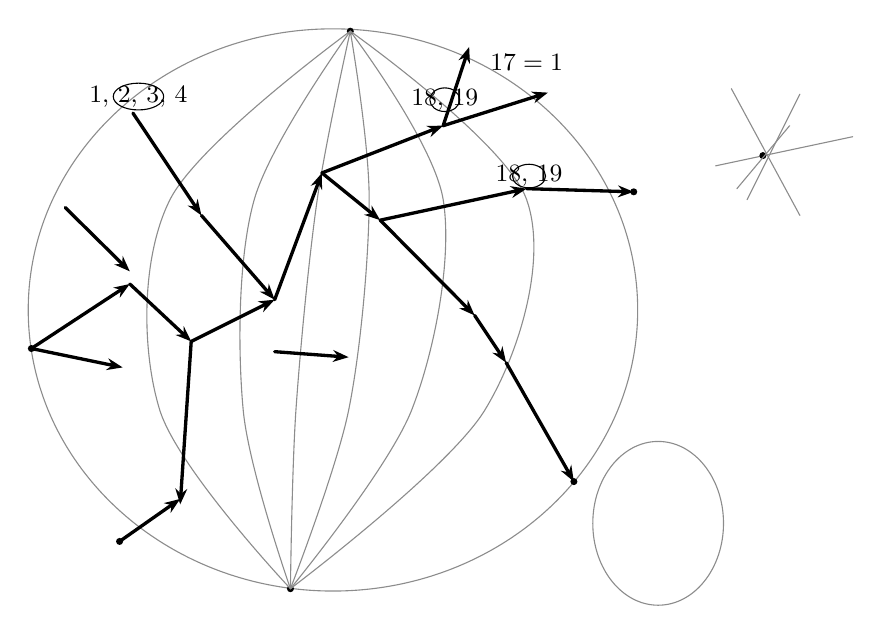
\begin{tikzpicture}[x=1mm,y=1mm,line cap=round,line join=round,font=\scriptsize]
\draw[pencil] (42.6,-42.3) ellipse[x radius=38.7, y radius=35.7];
\node[pt] at (44.8,-6.9) {};
\node[pt] at (37.2,-77.7) {};
\draw[pencil] plot[smooth, tension=0.55] coordinates {(44.8,-6.9) (21.9,-28.3) (20.6,-55) (37.2,-77.7)};
\draw[pencil] plot[smooth, tension=0.55] coordinates {(44.8,-6.9) (32.6,-28.3) (31.2,-55) (37.2,-77.7)};
\draw[pencil] plot[smooth, tension=0.55] coordinates {(44.8,-6.9) (40.6,-28.3) (37.9,-55) (37.2,-77.7)};
\draw[pencil] plot[smooth, tension=0.55] coordinates {(44.8,-6.9) (47.2,-28.3) (44.6,-55) (37.2,-77.7)};
\draw[pencil] plot[smooth, tension=0.55] coordinates {(44.8,-6.9) (56.6,-28.3) (52.6,-55) (37.2,-77.7)};
\draw[pencil] plot[smooth, tension=0.55] coordinates {(44.8,-6.9) (67.2,-28.3) (61.9,-55) (37.2,-77.7)};
\node[pt] at (4.3,-47.2) {};
\draw[very thick,-{Stealth[length=2mm]}] (4.3,-47.2) -- (16.8,-39);
\draw[very thick,-{Stealth[length=2mm]}] (4.3,-47.2) -- (15.9,-49.6);
\draw[very thick,-{Stealth[length=2mm]}] (8.6,-29.3) -- (16.8,-37.4);
\draw[very thick,-{Stealth[length=2mm]}] (17.2,-17.3) -- (25.9,-30.3);
\draw[very thick,-{Stealth[length=2mm]}] (25.9,-30.3) -- (35.2,-41);
\draw[very thick,-{Stealth[length=2mm]}] (16.8,-39) -- (24.6,-46.3);
\draw[very thick,-{Stealth[length=2mm]}] (24.6,-46.3) -- (35.2,-41);
\draw[very thick,-{Stealth[length=2mm]}] (35.2,-41) -- (41.2,-24.9);
\draw[very thick,-{Stealth[length=2mm]}] (41.2,-24.9) -- (48.6,-30.9);
\draw[very thick,-{Stealth[length=2mm]}] (48.6,-30.9) -- (67.2,-26.9);
\draw[very thick,-{Stealth[length=2mm]}] (41.2,-24.9) -- (56.6,-18.9);
\draw[very thick,-{Stealth[length=2mm]}] (56.6,-18.9) -- (69.9,-14.7);
\draw[very thick,-{Stealth[length=2mm]}] (56.6,-18.9) -- (59.9,-8.9);
\draw[very thick,-{Stealth[length=2mm]}] (48.6,-30.9) -- (60.6,-43);
\draw[very thick,-{Stealth[length=2mm]}] (60.6,-43) -- (64.6,-49);
\draw[very thick,-{Stealth[length=2mm]}] (64.6,-49) -- (73.2,-64.1);
\draw[very thick,-{Stealth[length=2mm]}] (24.6,-46.3) -- (23.2,-67);
\draw[very thick,-{Stealth[length=2mm]}] (15.5,-71.7) -- (23.2,-66.3);
\draw[very thick,-{Stealth[length=2mm]}] (67.2,-26.9) -- (80.8,-27.3);
\draw[very thick,-{Stealth[length=2mm]}] (35.2,-47.6) -- (44.6,-48.3);
\node[pt] at (15.5,-71.7) {};
\node[pt] at (80.8,-27.3) {};
\node[pt] at (73.2,-64.1) {};
\draw (17.9,-15.2) ellipse[x radius=3.2, y radius=1.7];
\node[inner sep=1pt] at (17.9,-15.2) {\small 1, 2, 3, 4};
\draw (56.8,-15.6) ellipse[x radius=1.9, y radius=1.5];
\node[inner sep=1pt] at (56.8,-15.6) {\small 18, 19};
\draw (67.5,-25.3) ellipse[x radius=2.1, y radius=1.5];
\node[inner sep=1pt] at (67.5,-25.3) {\small 18, 19};
\node[inner sep=1pt] at (67.2,-10.9) {\small $17=1$};
\draw[pencil] (91.2,-24) -- (108.6,-20.3);
\node[pt] at (97.2,-22.7) {};
\draw[pencil] (93.2,-14.2) -- (101.9,-30.3);
\draw[pencil] (101.9,-14.9) -- (95.2,-28.3);
\draw[pencil] (93.9,-26.9) -- (100.6,-18.9);
\draw[pencil] (83.9,-69.4) ellipse[x radius=8.3, y radius=10.4];
\end{tikzpicture}
\end{document}
